% pyformex manual --- tutorial
% $Id$
% (C) B.Verhegghe

\chapter{pyFormex tutorial}
\label{cha:tutorial}


%%
\section{The \pyf philosophy}
\label{sec:intro-tut}

\pyformex is a Python implementation of Formex algebra. Using \pyformex, it is very easy to generate large geometrical models of 3D structures by a sequence of mathematical transformations. It is especially suited for the automated design of spatial structures. But it can also be used for other tasks, like operating on 3D geometry obtained from other sources, or for finite element pre- and postprocessing, or just for creating some nice pictures.

By writing a simple script, a large and complex geometry can be created by copying, translating, rotating, or otherwise transforming geometrical entities. \pyformex will interpret the script and draw what you have created. This is clearly very different from the traditional (mostly interactive) way of creating a geometrical model, like is done in most CAD packages. There are some huge advantages in using \pyformex:
\begin{itemize}
\item It is especially suited for the automated design of spatial frame structures. A dome, an arc, a hypar shell, \dots, when constructed as a space frame, can be rather difficult and tedious to draw with a general CAD program; using scripted mathematical transformations however, it may become a trivial task.
\item Using a script makes it very easy to apply changes in the geometry: you simply modify the script and let \pyformex re-execute it. You can easily change any geometrical parameter in any way you want: set directly, interactively ask the user, calculate from some formula, read from a file, \dots.  angle, the radius of a dome, the ratio $f/l$ of an arc. Using CAD, you would have often have to completely redo your drawing work. This idea of scripted geometry building is illustrated in figure~\ref{fig:scallops}: all these domes were created with the same script, but with different values of some parameters.
\begin{figure}[ht]
  \centering
  \begin{makeimage}
  \end{makeimage}
  \begin{latexonly}
    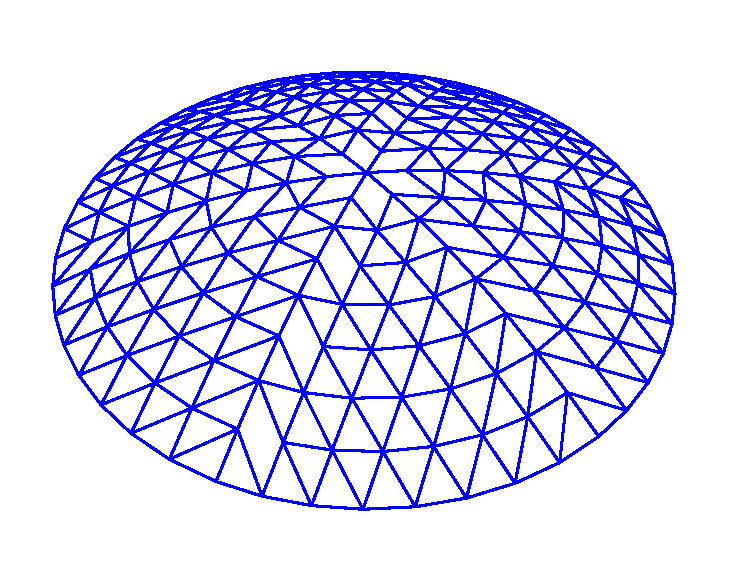
\includegraphics[width=5cm]{images/scallopdome-000}
    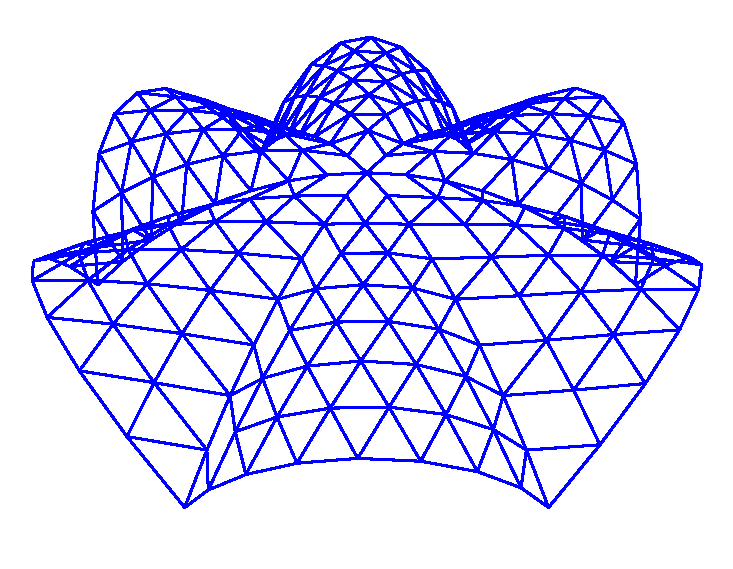
\includegraphics[width=5cm]{images/scallopdome-001}
    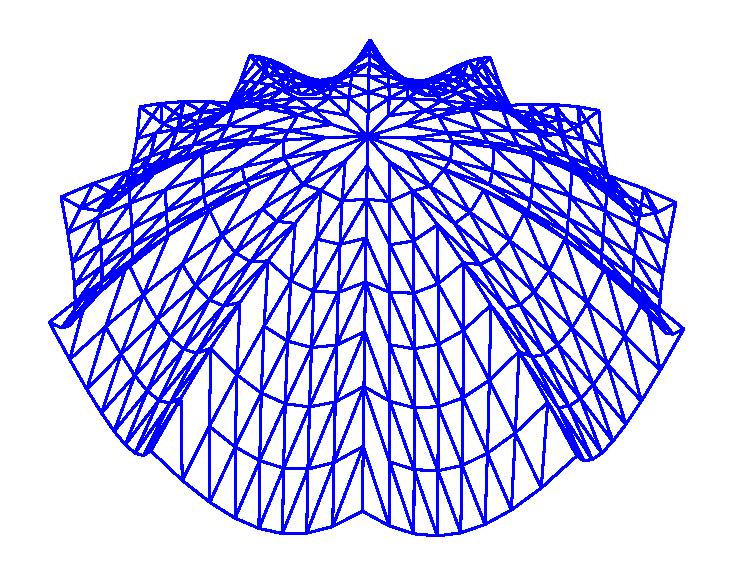
\includegraphics[width=5cm]{images/scallopdome-002}
  \end{latexonly}
  \begin{htmlonly}
    \htmladdimg{../images/scallopdome-000.png}
    \htmladdimg{../images/scallopdome-001.png}
    \htmladdimg{../images/scallopdome-002.png}
  \end{htmlonly}
  \caption{Same script, different domes} \label{fig:scallops}
\end{figure}
\item At times there will be operations that are easier to perform through an interactive Graphical User Interface (GUI). The \pyf GUI gives access to many of its functions. Especially occasional and untrained users will benefit from it. As everything else in \pyf, the GUI is completely open and can be modified at will by the user's application scripts, to provide an interface with either extended or restructed functionality.
\end{itemize}

% As mentioned, \pyformex is based on the programming language Python \footnote{\url{http://www.python.org}}. This implies that the scripts are also Python-based. It's a very easy language, but if you're interested in reading more, there is a very good tutorial available on \url{http://docs.python.org/tut/}. However, if you're only using Python to write \pyformex-scripts, the tutorial you're reading right now should be enough. 


%%%%%%%%%%%%%%%%%%%%%%%%%%%%%%%%%%%%%%%%%%%%%%%%%%%%%%%%%%%%%%%%%%%
\section{Getting started}
\label{sec:getting-started}

\outdated

\worktodo{This should include a short introduction to Python and Numpy}   

This section holds some basic information on how to use Python and \pyformex. 

\begin{itemize}
\item Start the \pyformex GUI by entering the command \emph{pyformex} in a terminal. Depending on your instalation, there may also be a menu item in the application menu to start \pyf, or even a quickstart button in the panel. Using the terminal however can still be useful, especially in the case of errors, because otherwise the GUI might suppress some of the error messages that normally are sent to the terminal.
\item To create a new \pyformex-script, just open a new file with your favorite text editor and save it under a name with extension '.py'.
\item A \pyf script should start with a line \Code{\#!/usr/bin/env pyformex}
\item To edit the script, you can
	\begin{itemize}
	\item open it with your favorite text editor.
	\item \menuselection{File \sub Open}\\
	At this point, the script will be loaded but nothing will happen. \\
	\menuselection{File \sub Edit}\\
	The script will now open in the default text editor. This default editor can be changed in the user configuration file (\file{~/.pyformexrc}) or using the \menuselection{Settings \sub Commands} menu option.
	\end{itemize}
\item To play a script, you can
	\begin{itemize}
	\item \menuselection{File \sub Open}\\
		\menuselection{File \sub Play} 
	\item Type \emph{pyformex myproject.py} in the terminal. This will start the \pyformex GUI and load your script at the same time. \\
\menuselection{File \sub Play}
	\item To play a script without using the GUI (for example in finite element preprocessing, if you only want to write an 		output file, without drawing the structure), type \emph{pyformex --nogui myproject.py}
	\end{itemize}
\item When writing a script in Python, there are some things you should keep in mind:
	\begin{itemize}
	\item When using a function that requires arguments, an argument list must have any positional arguments followed by any keyword arguments, where the keywords must be chosen from the formal parameter names. It's not important whether a formal parameter has a default value or not. No argument may receive a value more than once -- formal parameter names corresponding to positional arguments cannot be used as keywords in the same calls. 

Simply put: you can either set the arguments in the right order and only give their value, or you can give arguments by their name and value. This last option holds some advantages: not only is it easier to check what you did, but sometimes a function has many arguments with default values and you only want to change a few.
If this isn't entirely clear yet, just look at the examples later in this tutorial or check the Python tutorial.
	\item Indentation is essential in Python. Indentation is Python's way of grouping statements. In straight-forward scripts, indentation is not needed (and forbidden!), but when using a for-statement for example, the body of the statement has to be indented. A small example might make this clear. Also notice the ':' 
\begin{verbatim}
	print 'properties'
	for key, item in properties.iteritems():
	    print key, item
\end{verbatim}
	\item If you want to use functions from a seperate module (like \module{properties}), you add a line on top of the script
\begin{verbatim}
	from properties import *
\end{verbatim}
All functions from that module are now available.
	\item The hash character, "\#", is used to start a comment in Python.
	\item Python is case sensative.
	\end{itemize}
\end{itemize}


%%%%%%%%%%%%%%%%%%%%%%%%%%%%%%%%%%%%%%%%%%%%%%%%%%%%%%%%%%%%%%%%%
\section{Creating geometrical models}
\label{sec:geom}

\subsection{The Formex data model}

The most important geometrical object in \pyf is the \class{Formex}\index{Formex} class. A \class{Formex} can describe a variety of geometrical objects: points, lines, surfaces, volumes. The most simple geometrical object is the point, which in three dimensions is only determined by its coordinates \code(x,y,z), which in \pyf will be numbered \code(0,1,2) for convenience. Higher order geometrical objects are defined by a collection of points. In \pyf terms, we call the number of points of an object its \emph{plexitude}\index{plexitude}. 

A Formex is a collection of geometrical objects of the same plexitude. The objects in the collection are called the \emph{elements}\index{element} of the \class{Formex}. A \class{Formex} whose elements have plexitude $n$ is also called an $n$-plex \class{Formex}. Internally, the coordinates of the points are stored in a numerical array\footnote{\pyf uses the NumPy \class{ndarray} as implementation of fast numerical arrays in Python.} with three dimensions. The coordinates of a single point are stored along the last axis (2) of the \class{Formex}; all the points of an element are stored along the second axis (1); different elements are stored along the first axis (0) of the \class{Formex}. The figure~\ref{fig:formex} schematizes the structure of a \class{Formex}. 

\begin{figure}[ht]
  \centering
  \begin{makeimage}
  \end{makeimage}
  \begin{latexonly}
    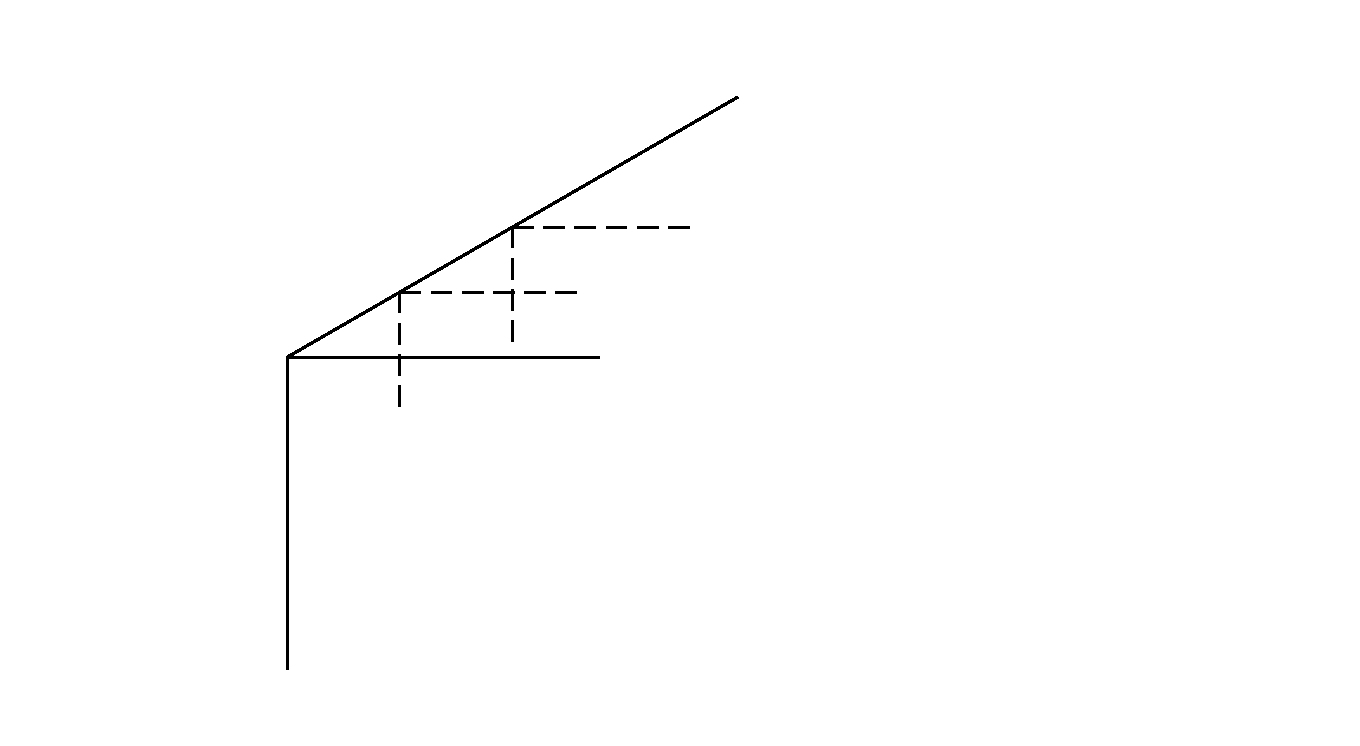
\includegraphics{images/Formex}
  \end{latexonly}
  \begin{htmlonly}
    \htmladdimg{../images/Formex.png}
  \end{htmlonly}  
  \caption{The structure of a Formex}
  \label{fig:formex}
\end{figure}

\warning{The beginning user should be aware not to confuse the three axes of a \class{Formex} with the axes of the 3D space. Both are numbered 0..2. The three coordinate axes form the components of the last axis of a Formex.}

For simplicity of the implemented algorithms, internally \pyf only deals with 3D geometry. This means that the third axis of a \class{Formex} always has length 3. You can however import 2D geometry: all points will be given a third coordinate $z=0.0$. If you restrict your operations to transformations in the $(x,y)$-plane, it suffices to extract just the first two coordinates to get the transformed 2D geometry.

The \class{Formex} object \code{F} can be indexed just like a $NumPy$ numerical array: \code{F[i]} returns the element with index $i$ (counting from $0$). For a \class{Formex} with plexitude $n$, the result will be an array with shape $(n,3)$, conttaining all the points of the element. Then, \code{F[i][j]} will be a $(3,)$-shaped array containing the coordinates of point $j$ of element $i$. Finally, \code{F[i][j][k]} is a floating point value representing a single coordinate of that point. 



%     A plane along the axes 2 and 1 is a set of points (F: cantle). This can be
%     thought of as a geometrical shape (2 points form a line segment, 3 points
%     make a triangle, ...) or as an element in FE terms. But it really is up to
%     the user as to how this set of points is to be interpreted.

%     Finally, the whole Formex represents a set of such elements.

%     Additionally, a Formex may have a property set, which is an 1-D array of
%     integers. The length of the array is equal to the length of axis 0 of the
%     Formex data (i.e. the number of elements in the Formex). Thus, a single
%     integer value may be attributed to each element. It is up to the user to
%     define the use of this integer (e.g. it could be an index in a table of
%     element property records).
%     If a property set is defined, it will be copied together with the Formex
%     data whenever copies of the Formex (or parts thereof) are made.
%     Properties can be specified at creation time, and they can be set,
%     modified or deleted at any time. Of course, the properties that are
%     copied in an operation are those that exist at the time of performing
%     the operation.   


\subsection{Creating a Formex}
\label{subsec:create}


\subsubsection{Creating a Formex using coordinates}
The first and most useful way to create a Formex is by specifying it's nodes and elements in a 3D-list.  

\begin{verbatim}
	F=Formex([[[0,0],[1,0],[1,1],[0,1]]])
\end{verbatim}

\begin{figure}[ht]
  \centering
  \begin{makeimage}
  \end{makeimage}
  \begin{latexonly}
    \includegraphics[width=4cm]{images/square}
  \end{latexonly}
  \begin{htmlonly}
    \htmladdimg{../images/square.png}
  \end{htmlonly}  
  \caption{A very simple Formex}
  \label{fig:square}
\end{figure}

This creates a Formex F, which has the nodes (0,0), (1,0), (1,1) and (0,1). These nodes are all part of a single element, thus creating a square plane. This element is also the entire Formex.
On the other hand, if you would change the position of the square brackets like in the following example, then you'd create a Formex F which is different from the previous. The nodes are the same, but the connection is different. The nodes (0,0) and (1,0) are linked together by an element, and so are the nodes (1,1) and (0,1). The Formex is now a set of 2 parallel bars, instead of a single square plane. 
\begin{verbatim}
	F=Formex([[[0,0],[1,0]],[[1,1],[0,1]]])
\end{verbatim}

\begin{figure}[ht]
  \centering
  \begin{makeimage}
  \end{makeimage}
  \begin{latexonly}
    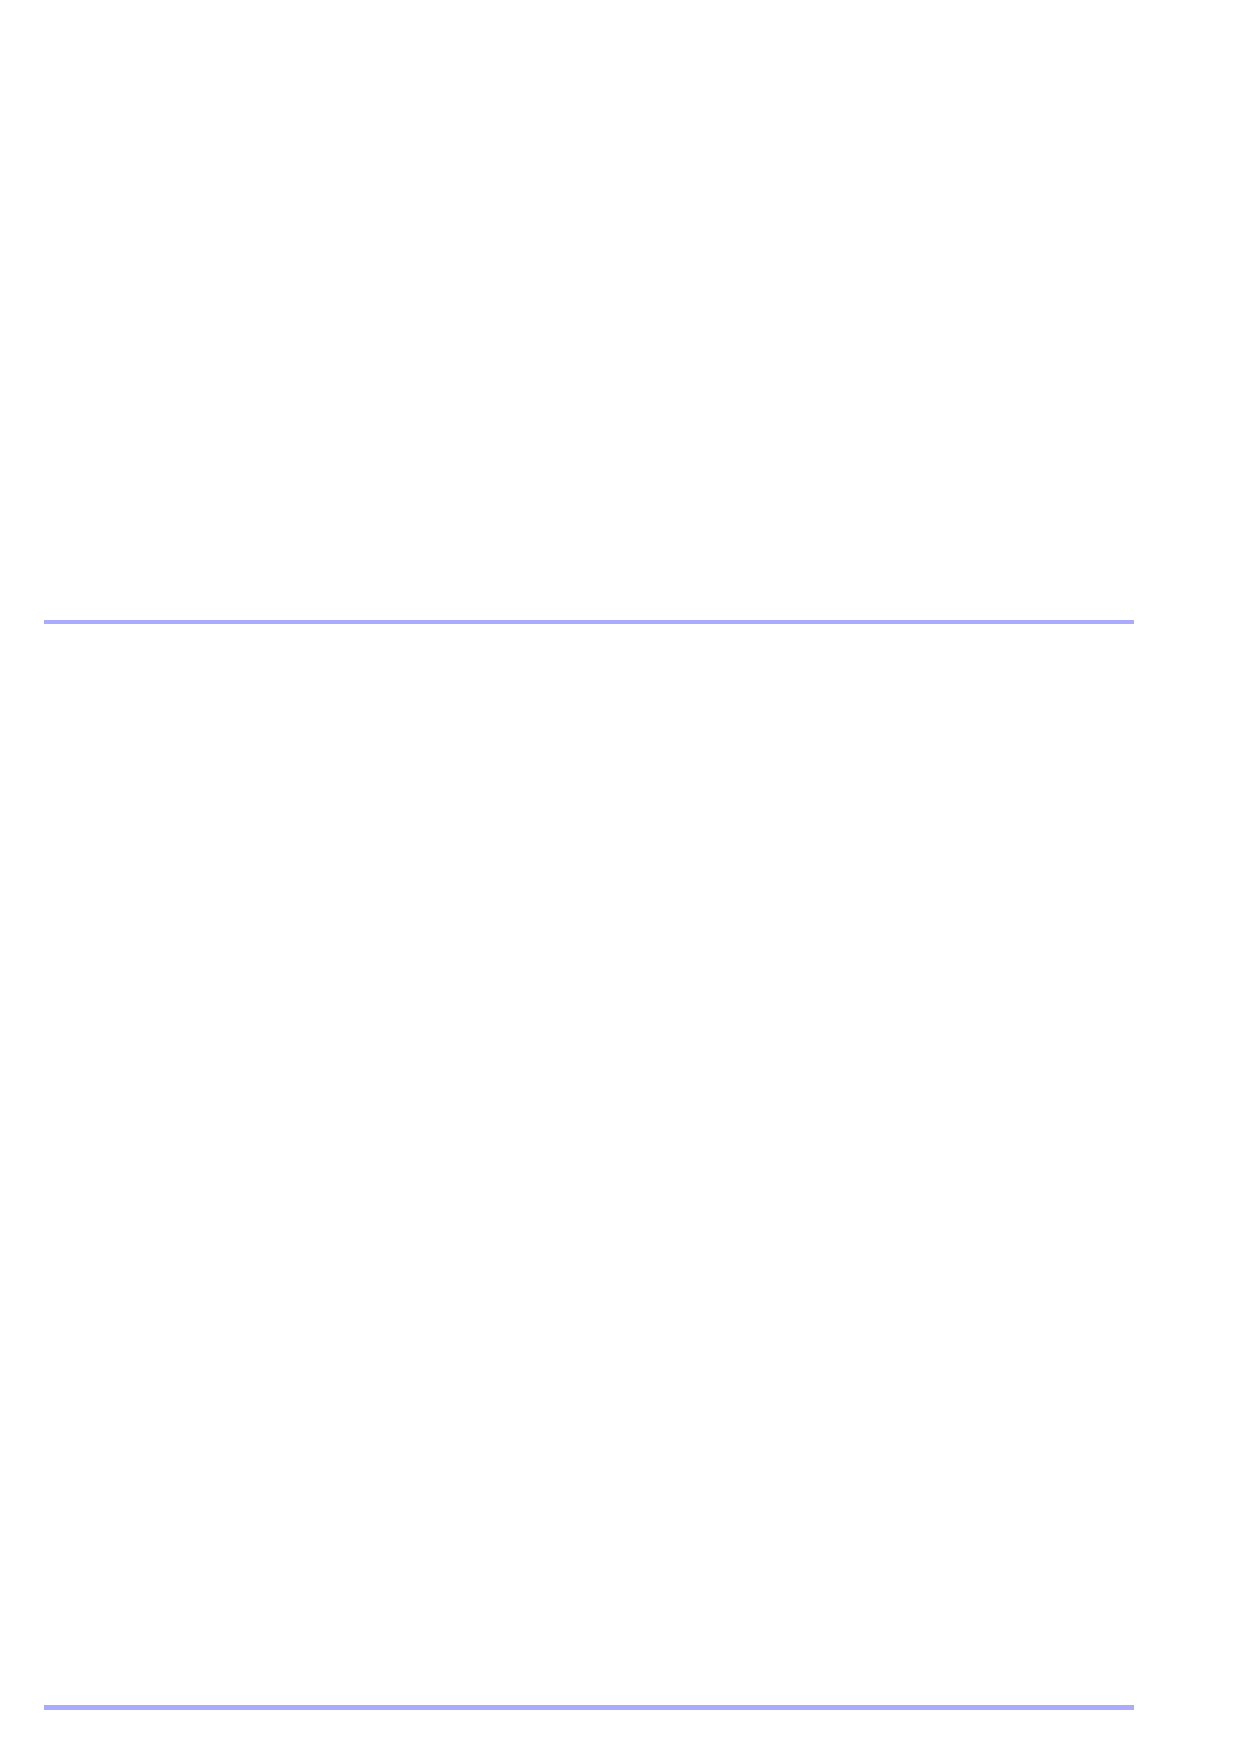
\includegraphics[width=4cm]{images/parallel}
  \end{latexonly}
  \begin{htmlonly}
    \htmladdimg{../images/parallel.png}
  \end{htmlonly}  
  \caption{Same nodes, different Formex}
\end{figure}

If we want to define a Formex, similar to the square plane, but consisting of the 4 edges instead of the actual plane, we have to define four elements and combine them in a Formex. This is \emph{not} the same Formex as fig \ref{fig:square}, although it looks exactly the same.
\begin{verbatim}
	F=Formex([[[0,0],[0,1]], [[0,1],[1,1]], [[1,1],[1,0]], [[1,0],[0,0]]])
\end{verbatim}

The previous examples were limited to a 2-D environment for simplicity's sake. Of course, we could add a third dimension. For instance, it's no problem defining a pyramid consisting of 8 elements ('bars').
\begin{verbatim}
	F=Formex([[[0,0,0],[0,1,0]], [[0,1,0],[1,1,0]], [[1,1,0],[1,0,0]], [[1,0,0], 
		[0,0,0]], [[0,0,0],[0,1,0]], [[0,0,0],[0.5,0.5,1]], [[1,0,0],[0.5,0.5,1]], 
		[[1,1,0], [0.5,0.5,1]], [[0,1,0],[0.5,0.5,1]]])
\end{verbatim}

\begin{figure}[ht]
  \centering
  \begin{makeimage}
  \end{makeimage}
  \begin{latexonly}
    \includegraphics[width=6cm]{images/pyramide}
  \end{latexonly}
  \begin{htmlonly}
    \htmladdimg{../images/pyramide.png}
  \end{htmlonly}  
  \caption{A pyramid}
  \label{fig:pyramid}
\end{figure}

However, as you can see, even in this very small example the number of nodes, elements and coordinates you have to declare becomes rather large. Defining large Formices using this method would not be practical. This problem is easily overcome by copying, translating, rotating,... a smaller Formex --- as will be explained in \ref{subsec:changing} --- or by using patterns.
 
\subsubsection{Creating a Formex using patterns}

Another way of creating a Formex, is by using the coordinate generating functions \function{pattern} and {mpattern}. These functions create a series of coordinates from a simple string, by interpreting each of the characters of the string as a single unit step in one of the cordinate directions, or as some other simple action. These functions thus are very valuable in creating geometry where the points lie on a regular grid.

 


In this case, a line segment pattern is created from a string.

The function \function{pattern(s)} creates a list of line segments where all nodes lie on the
gridpoints of a regular grid with unit step.
The first point of the list is [0,0,0]. Each character from the given
string \var{s} is interpreted as a code specifying how to move to the next node.
Currently defined are the following codes:\\
    0 = goto origin [0,0,0]\\
    1..8 move in the x,y plane\\
    9 remains at the same place\\
    When looking at the plane with the x-axis to the right,\\
    1 = East, 2 = North, 3 = West, 4 = South, 5 = NE, 6 = NW, 7 = SW, 8 = SE.\\
    Adding 16 to the ordinal of the character causes an extra move of +1 in
    the z-direction. Adding 48 causes an extra move of -1. This means that
    'ABCDEFGHI', resp. 'abcdefghi', correspond with '123456789' with an extra
    z +/-= 1.              
    The special character '\verb?\?' can be put before any character to make the
    move without making a connection.
    The effect of any other character is undefined.

This method has important restrictions, since it can only create lines on a regular grid. However, it can be a much easier and shorter way to define a simple Formex. This is illustrated by the difference in length between the previous creation of a square and the next one, although they define the same Formex (figure \ref{fig:square}).
\begin{verbatim}
	F=Formex(pattern('1234'))
\end{verbatim}

Some simple patterns are defined in \module{simple.py} and are ready for use. These patterns are stacked in a dictionary called 'Patterns'. Items of this dictionary can be accessed like \Code{Patterns['cube']}.
\begin{verbatim}
	#!/usr/bin/env pyformex
	from simple import *
	c=Formex(pattern(Pattern['cube']))
	clear();draw(c)
\end{verbatim}

\begin{figure}[ht]
  \centering
  \begin{makeimage}
  \end{makeimage}
  \begin{latexonly}
    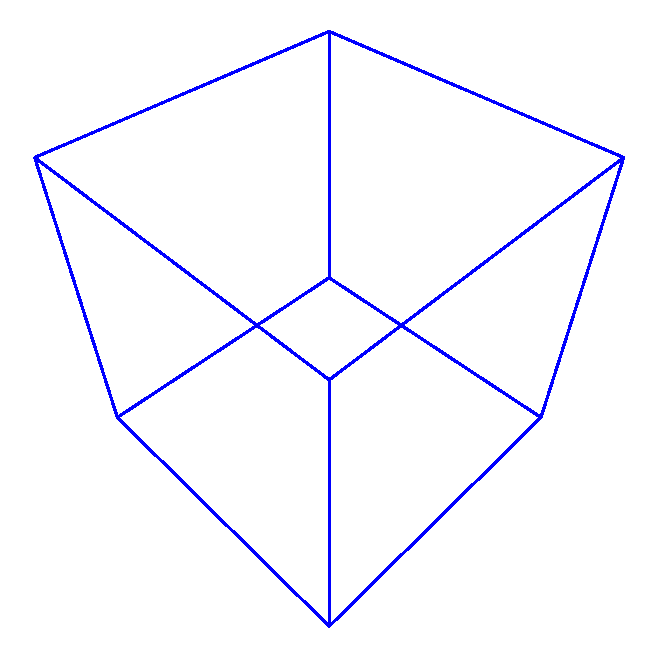
\includegraphics[width=6cm]{images/cube}
  \end{latexonly}
  \begin{htmlonly}
    \htmladdimg{../images/cube.png}
  \end{htmlonly}  
  \caption{A cube}
  \label{fig:cube}
\end{figure}


\subsubsection{Creating a Formex using coordinates from a file}
\outdated

In some cases, you might want to read coordinates from a file an combine them into a Formex. This is possible with the module \module{file2formex} and it's function \function{fileFormex()}. Each point is connected to the following, forming an element (bar).

The next file ('square.txt') would create the same square as before(figure \ref{fig:square}).
\begin{verbatim}
	0,0,0
	0,1,0
	1,1,0
	1,0,0
\end{verbatim}
\begin{verbatim}
	#!/usr/bin/env pyformex
	from file2formex import *
	F=fileFormex('square.text', closed='yes')
\end{verbatim}


\subsection{Drawing a Formex}
\outdated

\label{subsec:drawing}
Of course, you'd want to see what you have created. This is accomplished by the function \function{draw()}. The next example creates figure \ref{fig:pyramid}. 
\begin{verbatim}
	F=Formex([[[0,0,0],[0,1,0]], [[0,1,0],[1,1,0]], [[1,1,0],[1,0,0]], [[1,0,0], 
		[0,0,0]], [[0,0,0],[0,1,0]], [[0,0,0],[0.5,0.5,1]], [[1,0,0],[0.5,0.5,1]], 
		[[1,1,0], [0.5,0.5,1]], [[0,1,0],[0.5,0.5,1]]])
	draw(F)
\end{verbatim}

It also possible to draw multiple Formices at the same time.
\begin{verbatim}
	from simple import *
	F=Formex([[[0,0,0],[0,1,0]], [[0,1,0],[1,1,0]], [[1,1,0],[1,0,0]], [[1,0,0],
		[0,0,0]], [[0,0,0],[0,1,0]], [[0,0,0],[0.5,0.5,1]], [[1,0,0],[0.5,0.5,1]], 
		[[1,1,0],[0.5,0.5,1]], [[0,1,0],[0.5,0.5,1]]]).setProp(1)	
	G=Formex(pattern(Pattern['cube'])).setProp(3)
	draw(F+G)
\end{verbatim}
\begin{figure}[ht]
  \centering
  \begin{makeimage}
  \end{makeimage}
  \begin{latexonly}
    \includegraphics[width=6cm]{images/house}
  \end{latexonly}
  \begin{htmlonly}
    \htmladdimg{../images/house.png}
  \end{htmlonly}  
  \caption{Drawing multiple Formices}
  \label{fig:multiple}
\end{figure}
 
It might be important to realize that even if you don't draw a particular Formex, that doesn't mean you didn't create it!

Now, when you are creating a large geometry, you might be interested in seeing the different steps in the creation. To remove all previously drawn Formices, you can use \function{clear()}  what sweepes the screen clean. If you want to see a certain step in the creation longer than the default time, use \function{sleep(t)}, with \var{t} the delay (in seconds) before executing the next command.
\begin{verbatim}
	F=Formex(pattern('164'))
	draw(F)
	G=F.replic(5,1,0)
	clear()
	draw(G)
\end{verbatim}


\subsection{Adding property numbers}
\label{subsec:propnr}
Apart from the coordinates of its points, a Formex object can also store a set of property numbers. This is a set of integers, one for every element of the Formex.
The property numbers are stored in an attribute \member{p} of the Formex. They can be set, changed or deleted, and be used for any purpose the user wants, e.g. to number the elements in a different order than their appearence in the coordinate array. Or they can be used as pointers into a large database that stores all kind of properties for that element. Just remember that a Formex either has no property numbers, or a complete set of numbers: one for every element.

Property numbers can play an important role in the modelling process, because they present some means of tracking how the resulting Formex was created. Indeed, each transformation of a Formex that preserves its structure, will also preserve the property numbers. Concatenation of Formices with property numbers will also concatenate the property numbers. If any of the concatenated Formices does not have property numbers, it will receive value 0 for all its elements. If all concatenated Formices are without properties, so will be the resulting Formex.

On transformations that change the structure of the Formex, such as replication, each element of the created Formex will get the property number of Formex element it was generated from.

To create a Formex with property numbers, just specify them as a second argument in the constructor. The following example creates a Formex consisting of two triangles, one with property number 1, the second with property 3. The following lines show the creation of the four Formices displayed in figure~\ref{fig:props}, where elements with proprty value 1 are shown in red, those with property value 3 are shown in blue. 
\begin{verbatim}
>>> F0 = Formex(mpattern('12-34'),[1,3])
>>> F1 = F0.replic2(4,2)
>>> F2 = F1 + F1.mirror(1)
>>> F3 = F2 + F2.rotate(180.,1)
\end{verbatim}

\begin{figure}[ht]
  \centering
  \begin{makeimage}
  \end{makeimage}
  \begin{latexonly}
    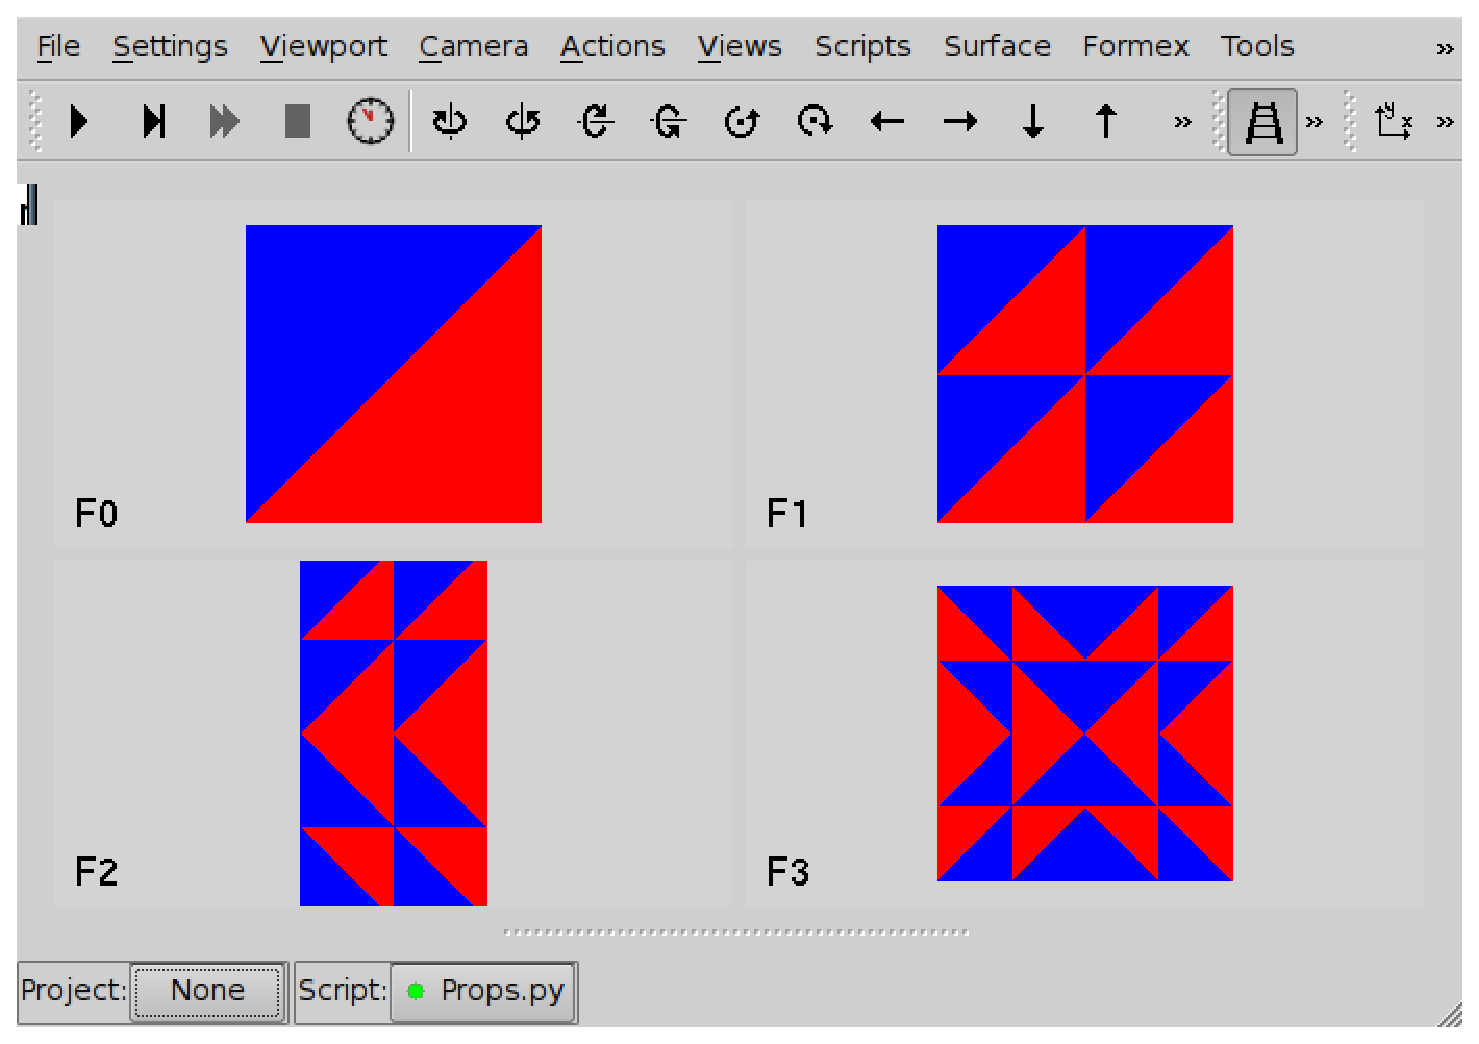
\includegraphics[width=10cm]{images/props}
  \end{latexonly}
  \begin{htmlonly}
    \htmladdimg{../images/props.png}
  \end{htmlonly}  
  \caption{A Formex with property numbers drawn as colors}
  \label{fig:props}
\end{figure}

To create the properties on a Formex without, you should always use the \method{setProp} method. This ensures that the properties array is generated with the correct type and shape. If needed, the supplied values will be repeated to match the number of elements in the Formex. Once the \member{p} attribute is created, you can safely change the value of any of the property numbers.
\begin{verbatim}
>>> F = Formex(mpattern('12-34-32-14'))
>>> F.setProp([1,3])
>>> print F.p
    [1 3 1 3]
>>> F.p[2] = 5
>>> print F.p
    [1 3 5 3]   
\end{verbatim}

When drawing a Formex having property numbers with default draw options (i.e. no color specified), pyFormex will use the property numbers as indices in a color table, so different properties are shown in different colors. The default color table has eight colors: \code{[ black, red, green, blue, cyan, magenta, yellow, white]} and will wrap around if a property value larger than 7 is used. You can however specify any other and larger colorset to be used for drawing the property colors.  



\subsection{Saving images}
\outdated

\label{subsec:images}
After drawing the Formex, you might want to save the image. This is very easy to do:\\
\menuselection{File \sub Save Image}\\
The filetype should be 'bmp', 'jpg', 'pbm', 'png', 'ppm', 'xbm', 'xpm', 'eps', 'ps', 'pdf' or 'tex'. \\
To create a better looking picture, several settings can be changed:
\begin{itemize}
	\item Change the background color \menuselection{Settings \sub Background Color}
	\item Use a different (bigger) linewidth \menuselection{Settings \sub Linewidth}
	\item Change the canvas size. This prevents having to cut and rescale the figure with an image manipulation program (and loosing quality by doing so).  \menuselection{Settings \sub Canvas Size}
\end{itemize}

It is also possible to save a series of images. This can be especially useful when playing a script which creates several images, and you would like to save them all.  For example, figure \ref{fig:WireStent-steps}, which shows the different steps in the creation of the WireStent model, was created this way.\\
\menuselection{File \sub Toggle MultiSave}\\


\subsection{Information about a Formex}
\label{subsec:info}

The Formex class has several methods related to abtaining information obout the object. We refer to the reference manual in chapter~\ref{cha:reference} for a full list. Some of the most interesting and often used ones are:
\begin{tableii}{l|l}{exception}{Function}{Description}
  \lineii{F.nelems()}{Return the number of elements in the Formex.}
  \lineii{F.nplex()}{Return the plexitude (the number of point in each element) of the Formex.}
  \lineii{F.prop()}{Return the properties array (same as F.p).}
  \lineii{F.bbox()}{Return the bounding box of the Formex.}
  \lineii{F.center()}{Return the center of the Formex.}
\end{tableii}

\subsection{Changing the Formex}
\label{subsec:changing}
Until now, we've only created simple Formices. The strength of \pyformex however is that it is very easy to generate large geometrical models by a sequence of mathematical transformations. After initiating a basic Formex, it's possible to transform it by using copies, translations, rotations, projections,...

There are many transformations available, but this is not the right place to describe them all. This is what the reference manual in chapter \ref{cha:reference} is for. A summary of all possible transformations and functions can be found there.

To illustrate some of these transformations and the recommended way of writing a script, we will analyse some of the examples. More of these interesting examples are found in \file{installdir/examples}. Let's begin with the example \file{Spiral.py}. 

\verbatiminput{scripts/Spiral.py}

During this first read-through, you will have noticed that every step is drawn. Of course, this is not necessary, but it can be useful. And above all, it is very educational for use in a tutorial...

The next important thing is that parameters were used. It's recommended to always do this, especially when you want to do a parametric study of course, but it can also be very convenient if at some point you want to change the geometry (for example when you want to re-use the script for another application).

A simple function \function{drawit()} is defined for use in this script only. This function only provides a shorter way of drawing Formices, since it combines \function{clear()} and \function{draw}. 

Now, let's dissect the script.

\begin{verbatim}
def drawit(F,view='front'):
    clear()
    draw(F,view)
\end{verbatim}
This is a small function that is only defined in this script. It clears the screen and draws the Formex at the same time. 

\begin{verbatim}
m = 36 # number of cells along torus big circle
n = 10 # number of cells along torus small circle
\end{verbatim}
These are the parameters. They can easily be changed, and a whole new spiral will be created without any extra effort.
The first step is to create a basic Formex. In this case, it's a triangle which has a different property number for every edge.
\begin{verbatim}
F = Formex(pattern("164"),[1,2,3]); drawit(F)  
\end{verbatim}
\begin{figure}[ht]
  \centering
  \begin{makeimage}
  \end{makeimage}
  \begin{latexonly}
    \includegraphics[width=6cm]{images/spiral-000}
  \end{latexonly}
  \begin{htmlonly}
    \htmladdimg{../images/spiral-000.png}
  \end{htmlonly}  
  \caption{The basic Formex}
\end{figure}

This basic Formex is copied 'm' times in the 0-direction with a translation 
step of '1' (the length of an edge of the triangle). After that, the new 
Formex is copied 'n' times in the 1-direction with a translation step of '1'. 
Because of the recursive definition (F=F.replic), the original Formex F is 
overwritten by the transformed one.
\begin{verbatim}
F = F.replic(m,1,0); drawit(F)
F = F.replic(n,1,1); drawit(F)
\end{verbatim}

Now a copy of this last Formex is translated in direction '2' with a 
translation step of '1'. This necessary for the transformation into a cilinder.
The result of all previous steps is a rectangular pattern with the desired 
dimensions, in a plane z=1.
\begin{verbatim}
F = F.translate(2,1); drawit(F,'iso')
\end{verbatim}
\begin{figure}[ht]
  \centering
  \begin{makeimage}
  \end{makeimage}
  \begin{latexonly}
    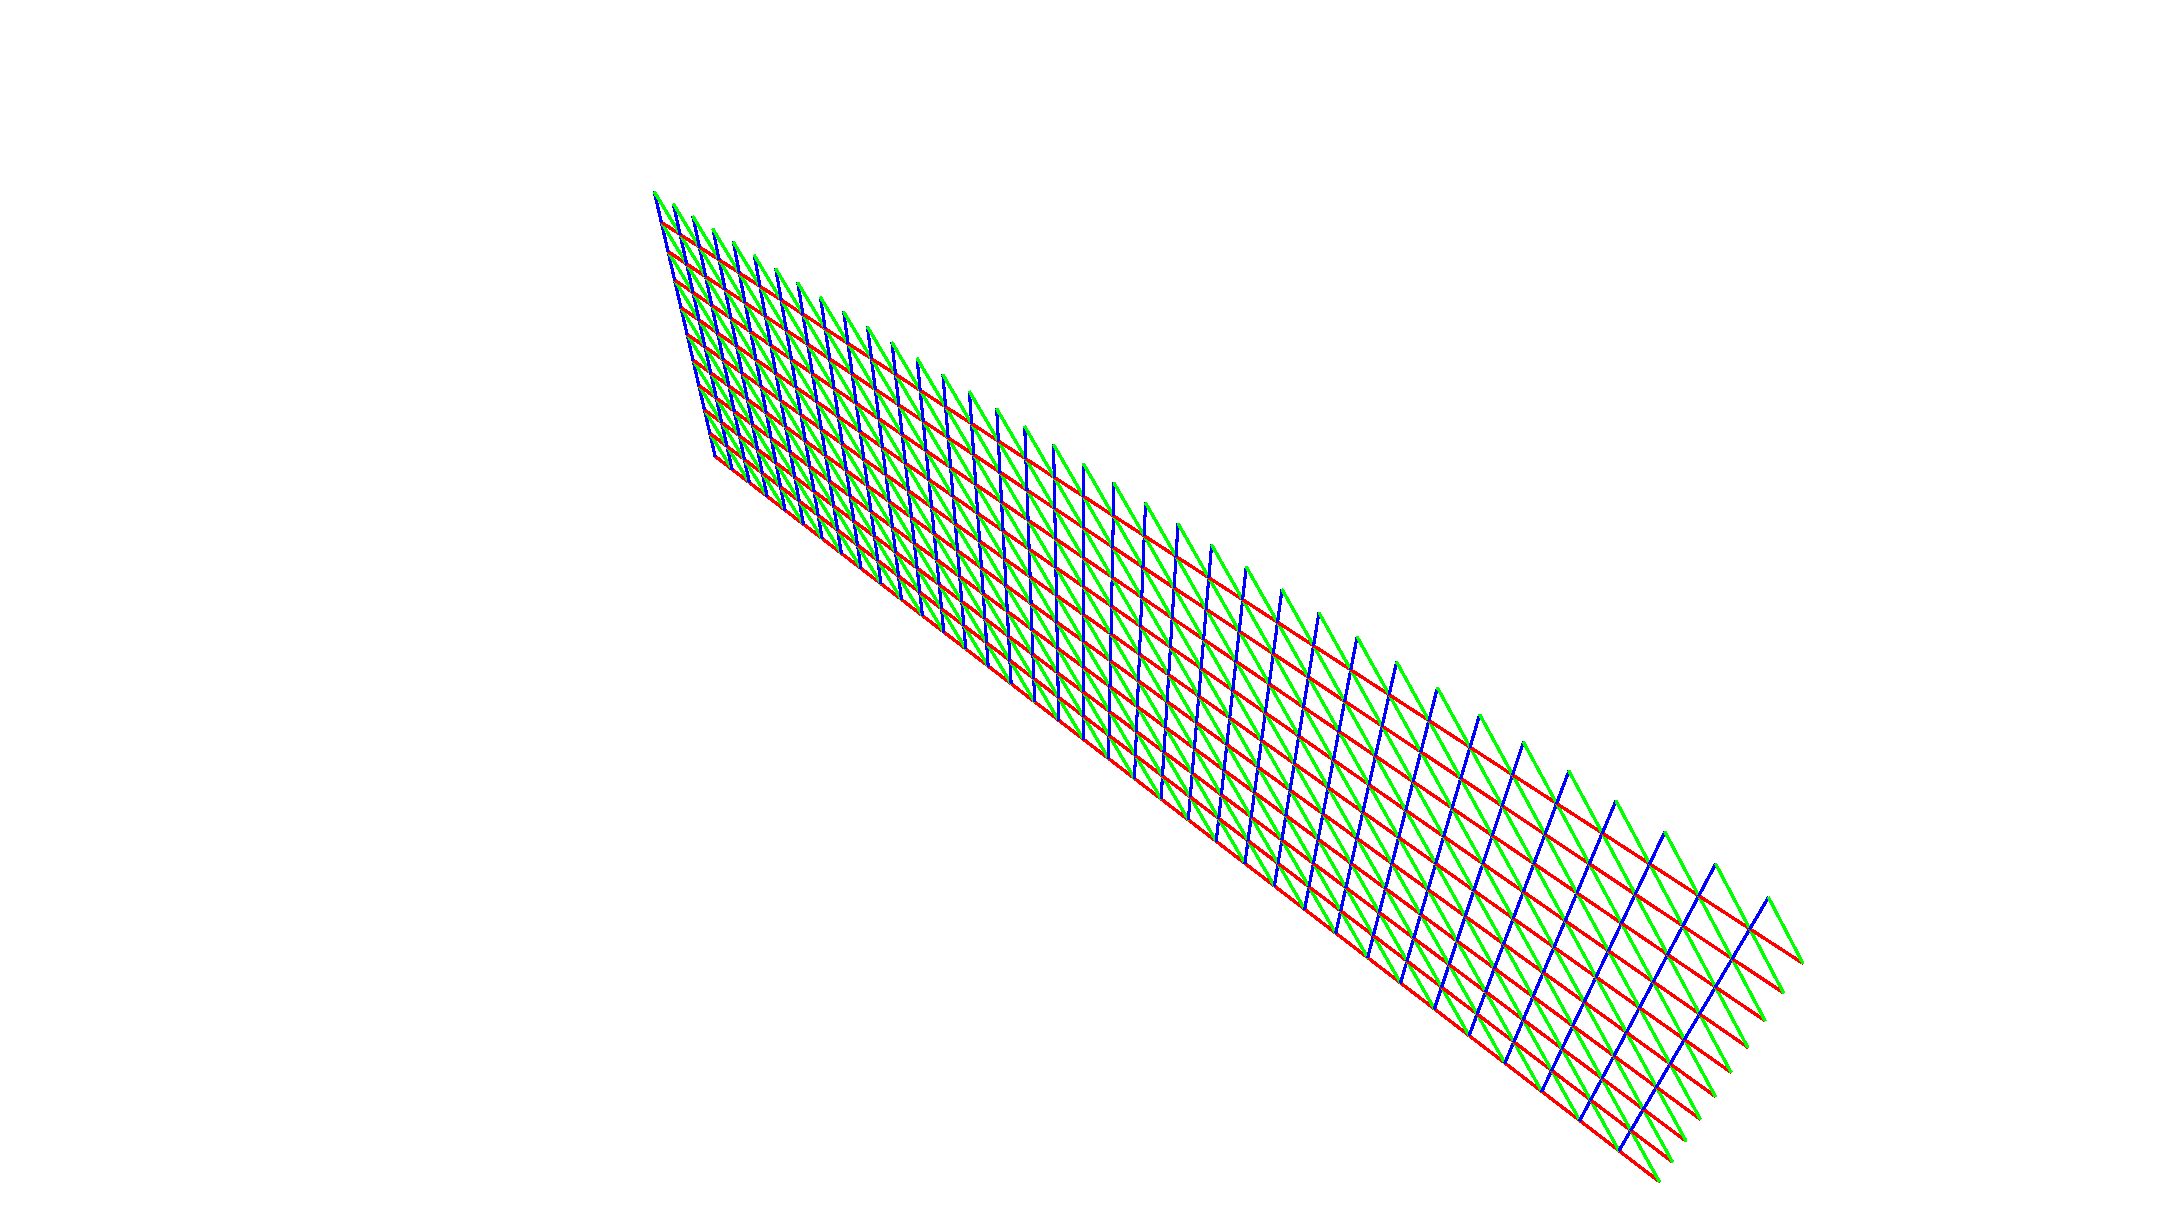
\includegraphics[width=6cm]{images/spiral-003}
  \end{latexonly}
  \begin{htmlonly}
    \htmladdimg{../images/spiral-003.png}
  \end{htmlonly}  
  \caption{The rectangular pattern}
\end{figure}

This pattern is rolled up into a cilinder around the 2-axis. 
\begin{verbatim}
F = F.cylindrical([2,1,0],[1.,360./n,1.]); drawit(F,'iso')
\end{verbatim}
\begin{figure}[ht]
  \centering
  \begin{makeimage}
  \end{makeimage}
  \begin{latexonly}
    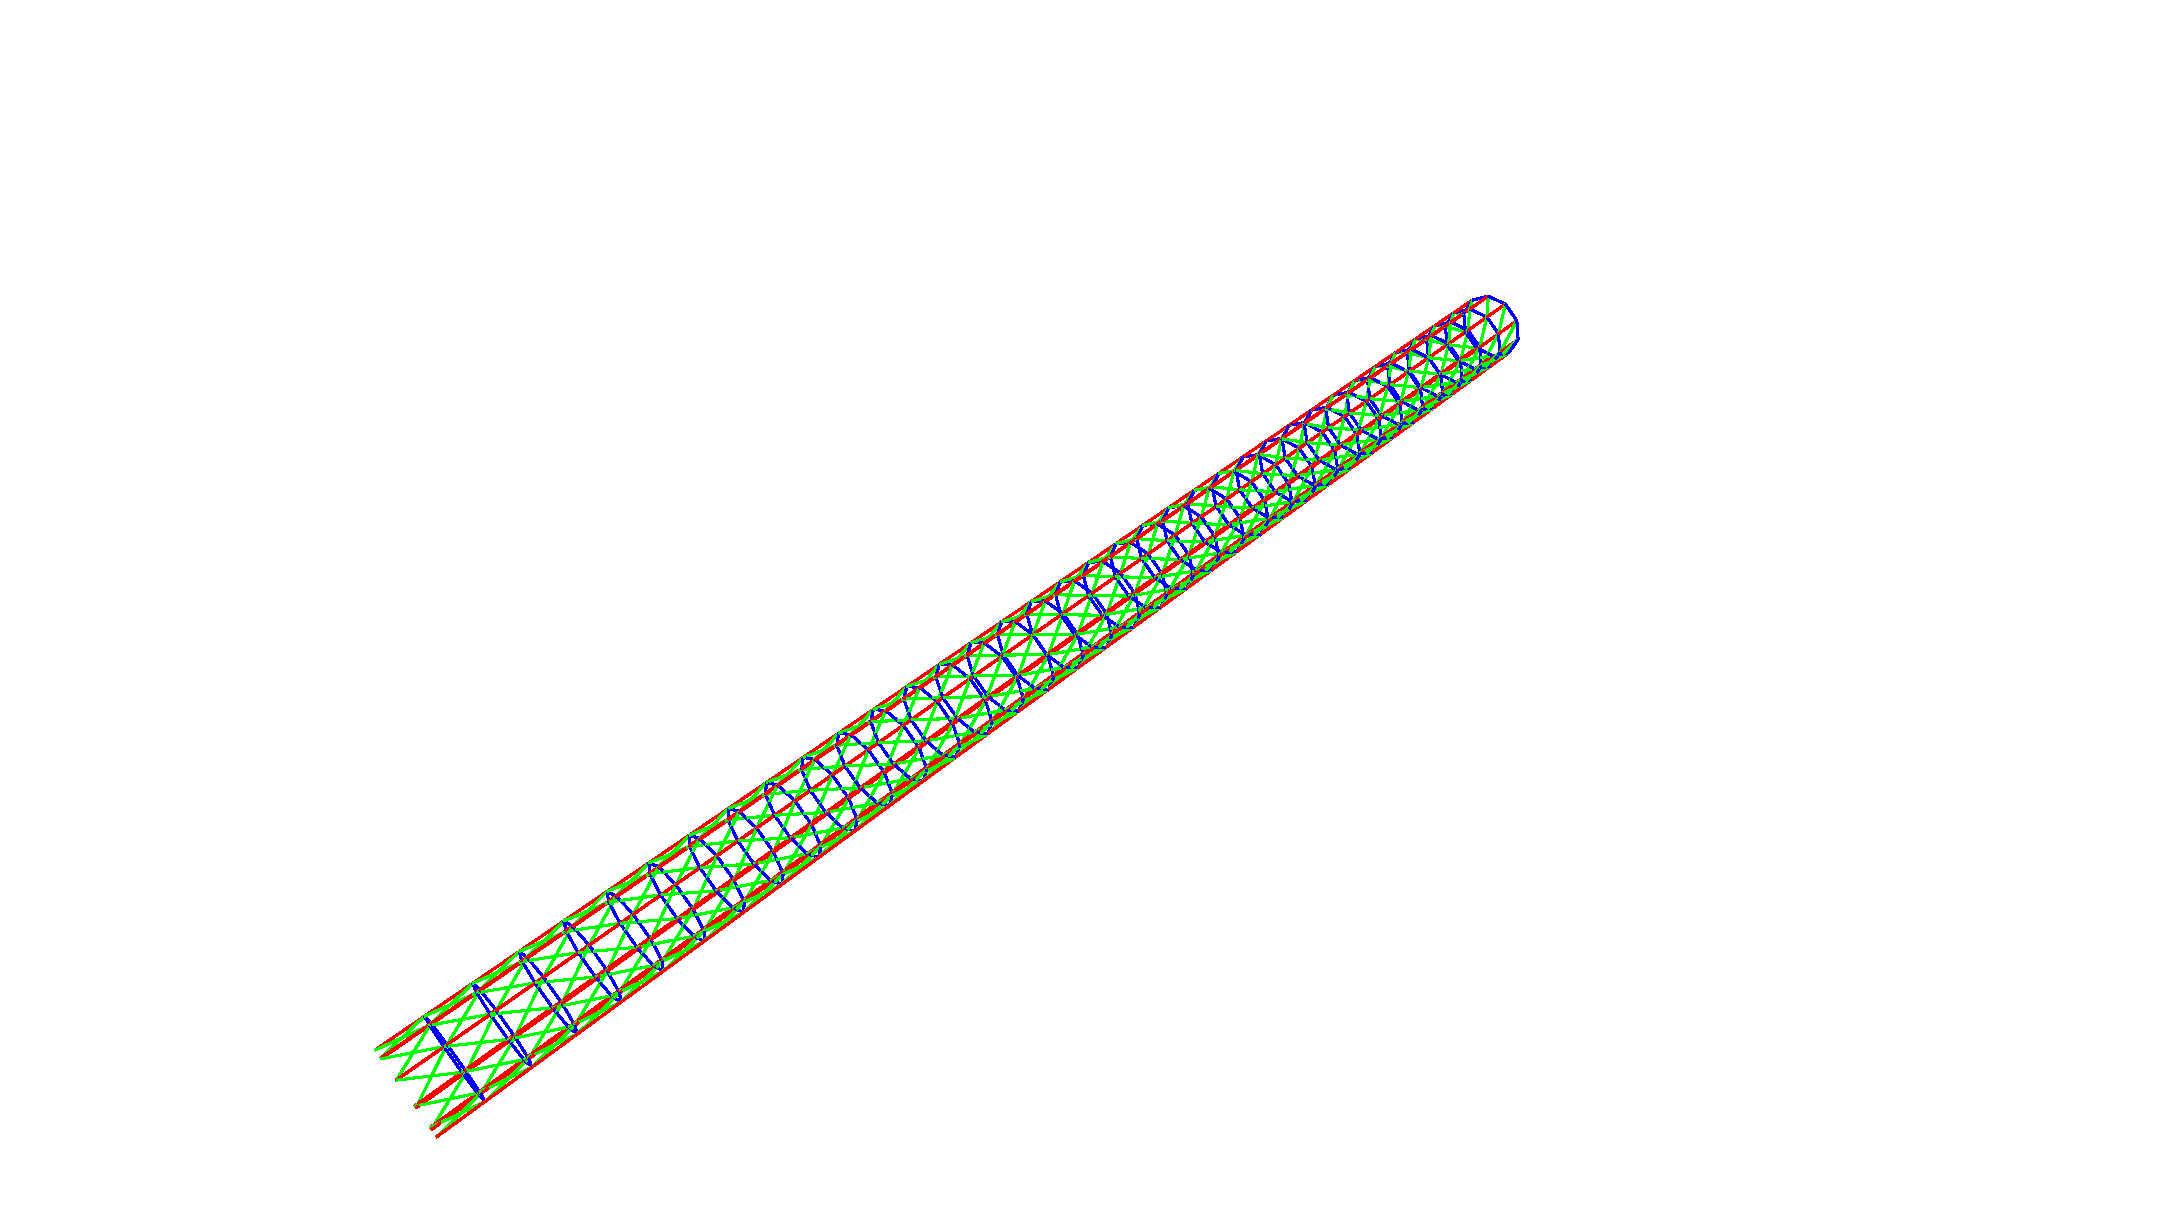
\includegraphics[width=6cm]{images/spiral-004}
  \end{latexonly}
  \begin{htmlonly}
    \htmladdimg{../images/spiral-004.png}
  \end{htmlonly}  
  \caption{The cylinder}
\end{figure}

This cilinder is copied 5 times in the 2-direction with a translation step of 
'm' (the lenght of the cilinder). 
\begin{verbatim}
F = F.replic(5,m,2); drawit(F,'iso')
\end{verbatim}

The next step is to rotate this cilinder -10 degrees around the 0-axis. 
This will determine the pitch angle of the spiral.
\begin{verbatim}
F = F.rotate(-10,0); drawit(F,'iso')
\end{verbatim}
\begin{figure}[ht]
  \centering
  \begin{makeimage}
  \end{makeimage}
  \begin{latexonly}
    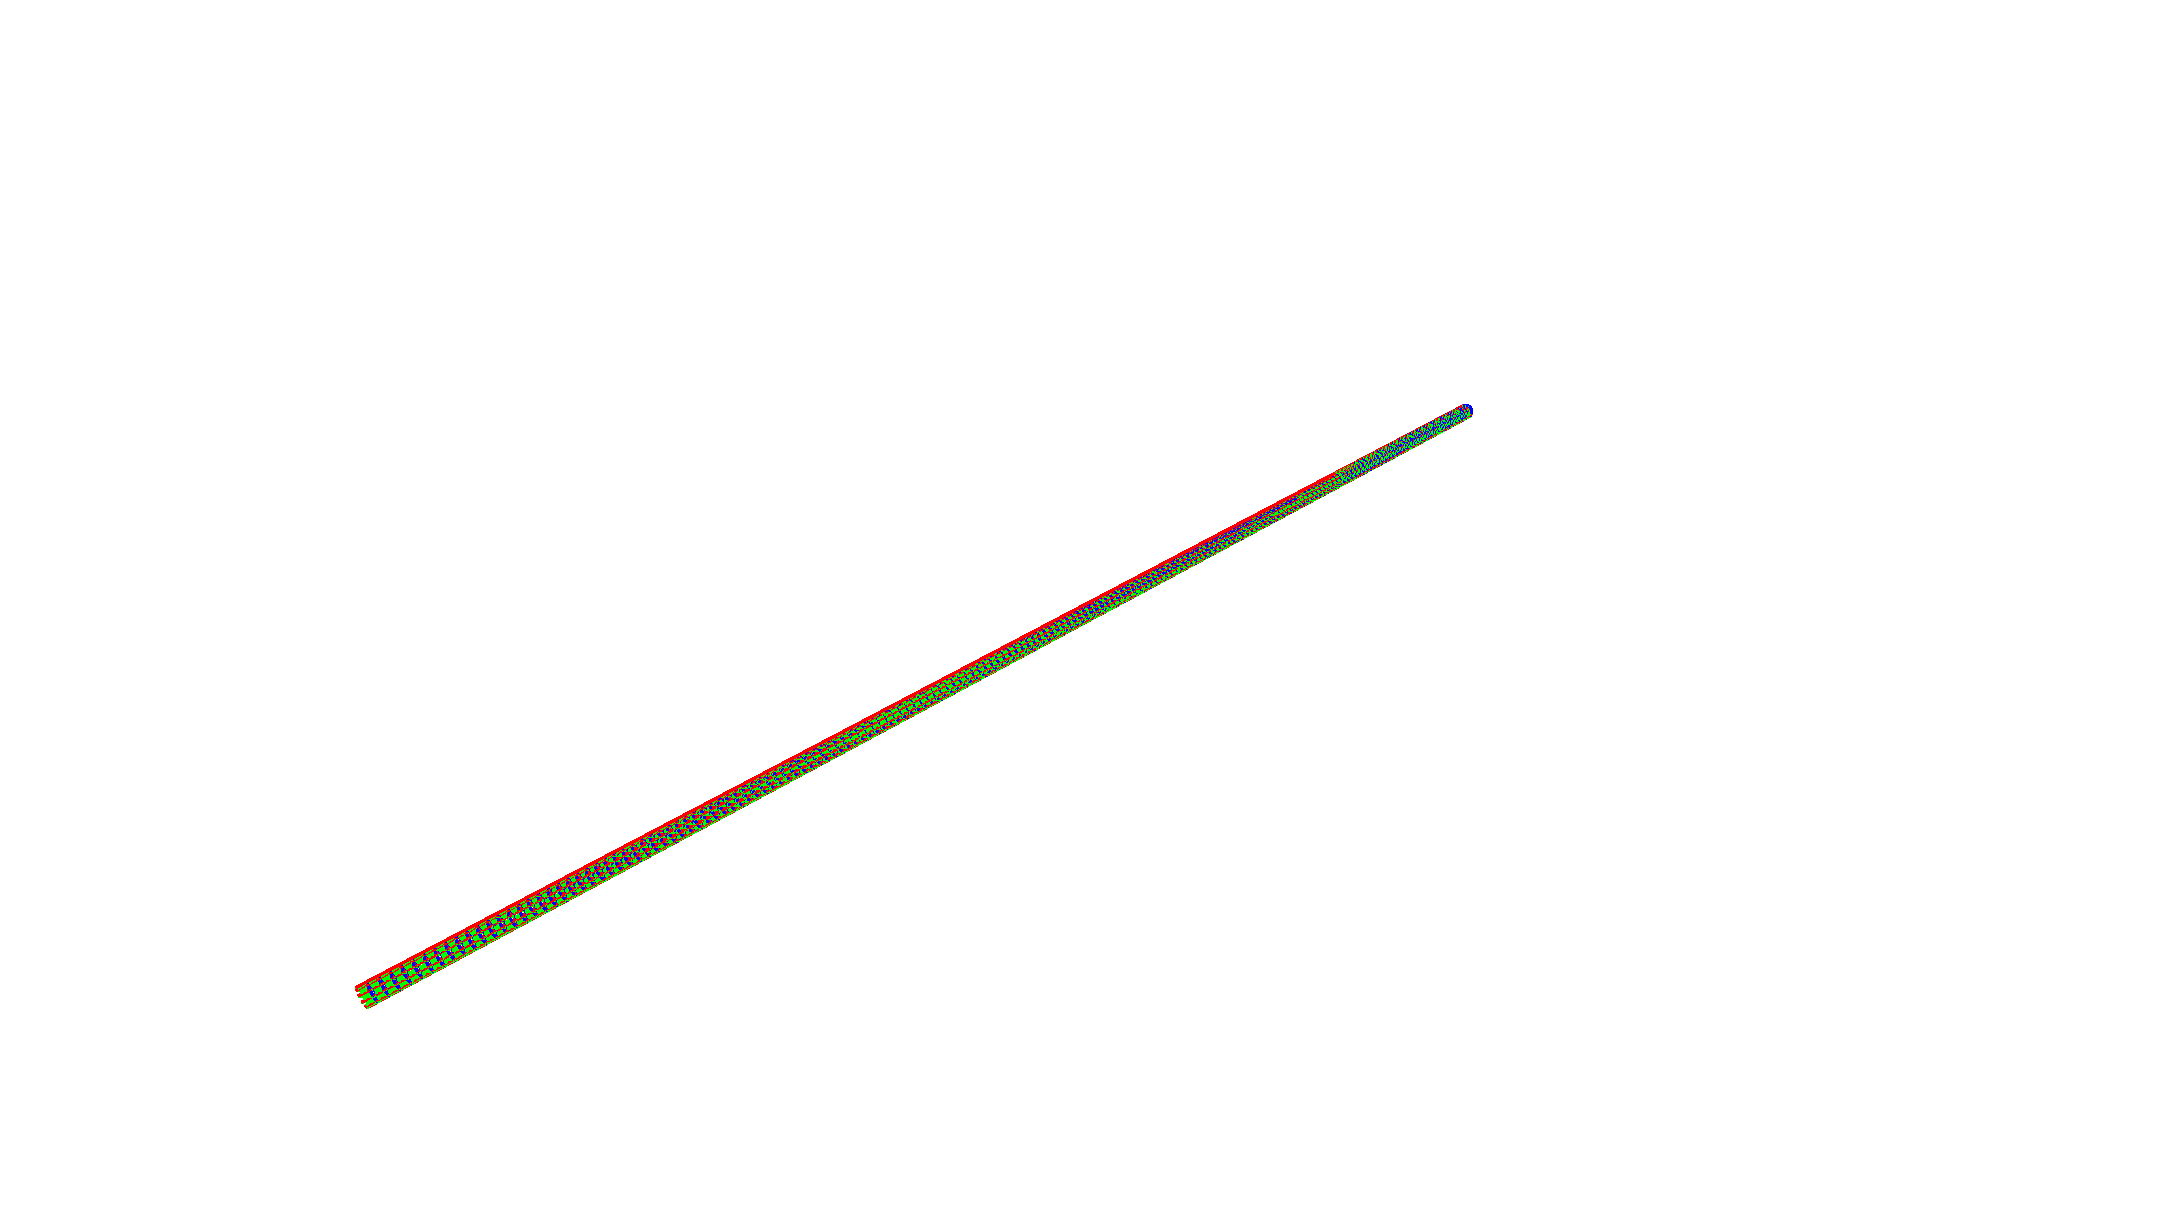
\includegraphics[width=6cm]{images/spiral-006}
  \end{latexonly}
  \begin{htmlonly}
    \htmladdimg{../images/spiral-006.png}
  \end{htmlonly}  
  \caption{The new cylinder}
\end{figure}

This last Formex is now translated in direction '0' with a translation step of '5'. 
\begin{verbatim}
F = F.translate(0,5); drawit(F,'iso')
\end{verbatim}

Finally, the Formex is rolled up, but around a different axis then before. 
Due to the pitch angle, a spiral is created. If the pitch angle would be 0 
(no rotation of -10 degrees around the 0-axis), the resulting Formex 
would be a torus. 
\begin{verbatim}
F = F.cylindrical([0,2,1],[1.,360./m,1.]); drawit(F,'iso')
drawit(F,'right')
\end{verbatim}

\begin{figure}[ht]
  \centering
  \begin{makeimage}
  \end{makeimage}
   \begin{latexonly}
     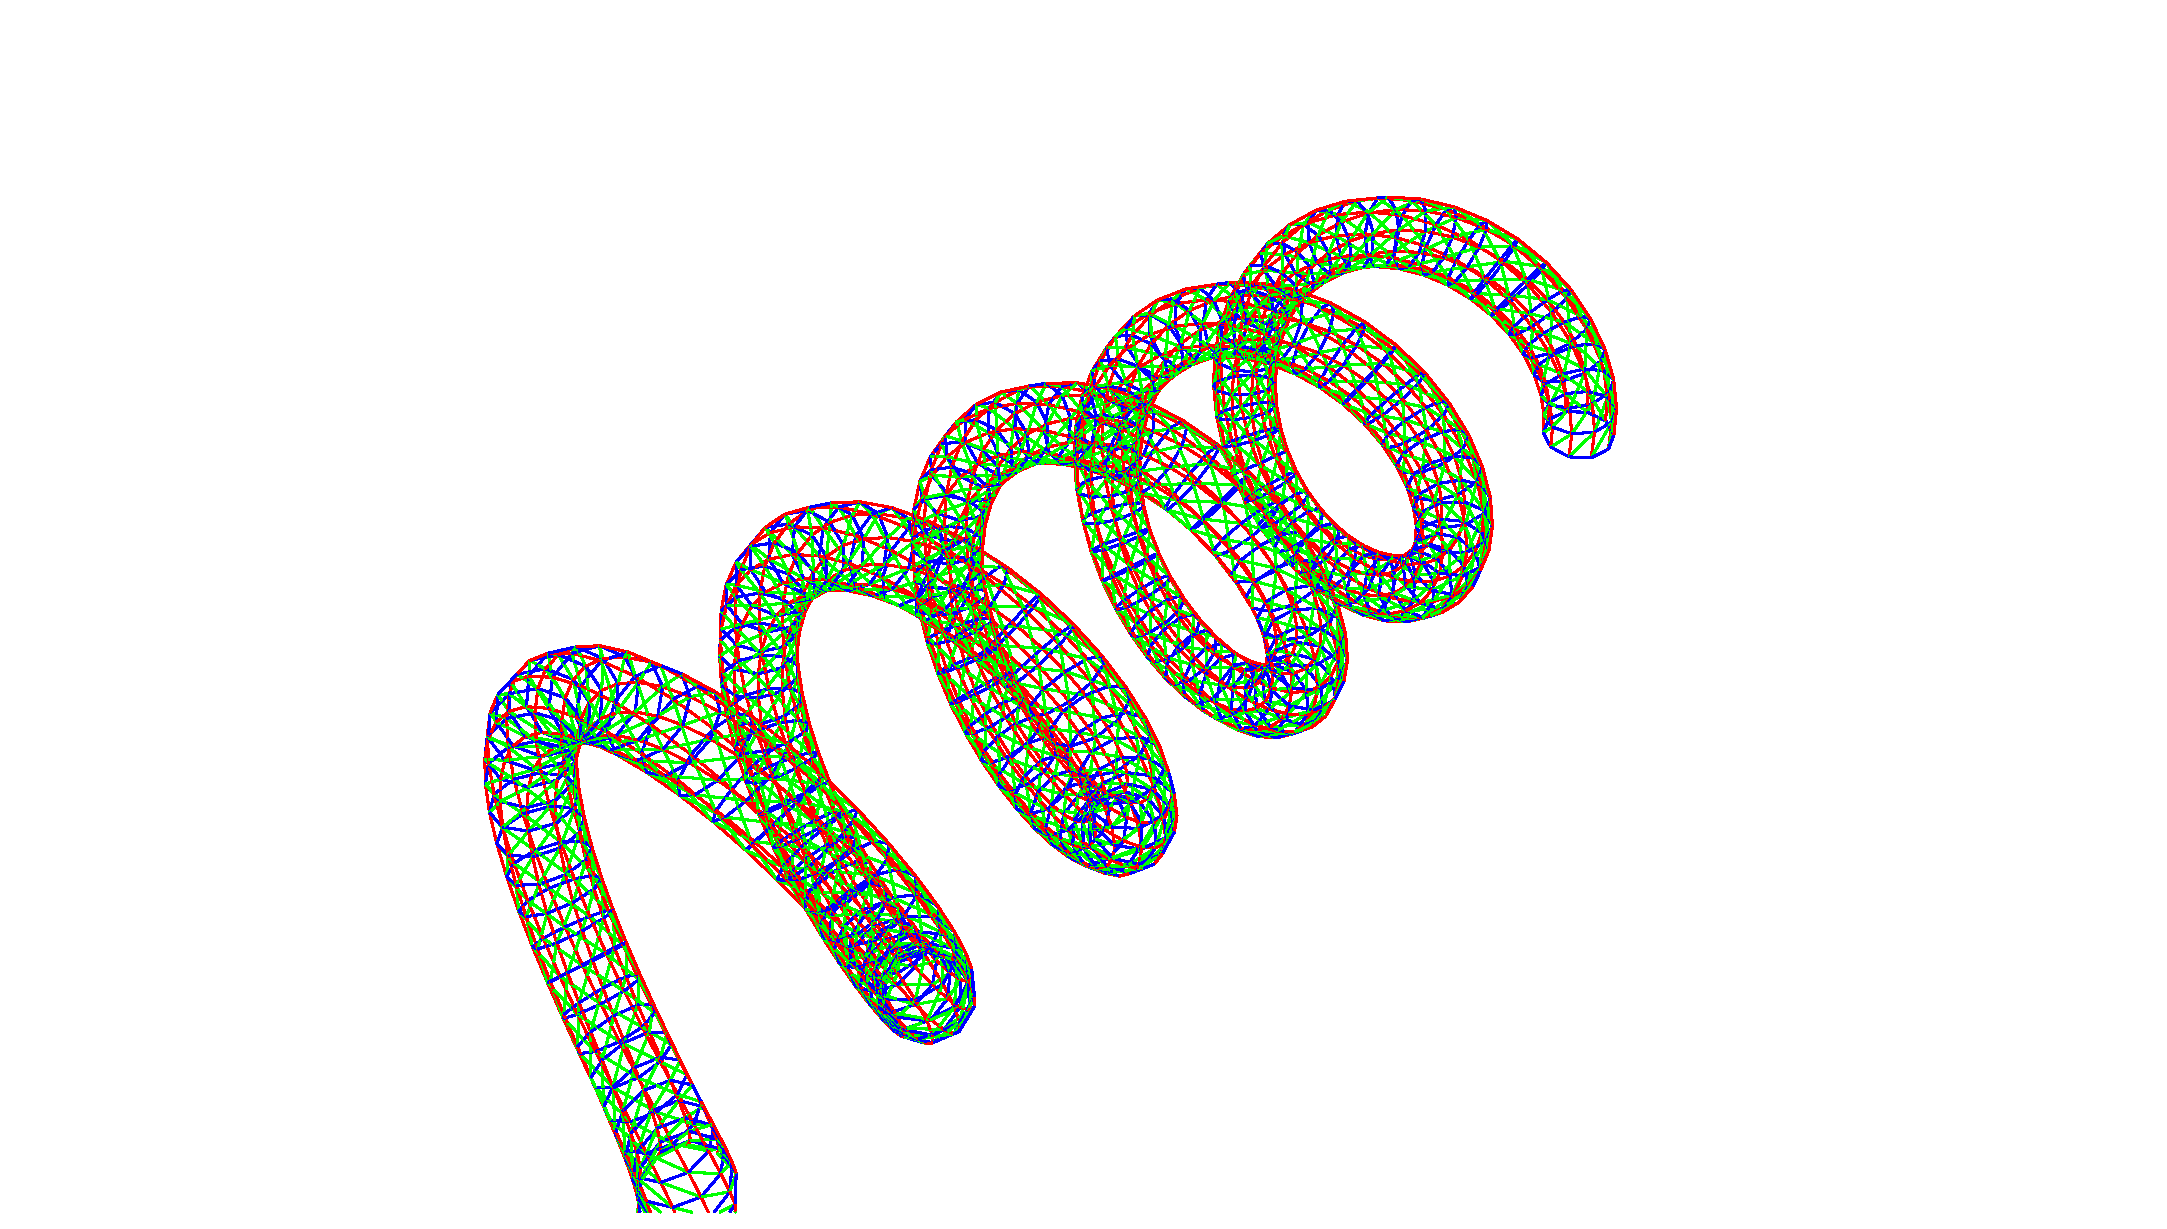
\includegraphics[width=5cm]{images/spiral-007}
     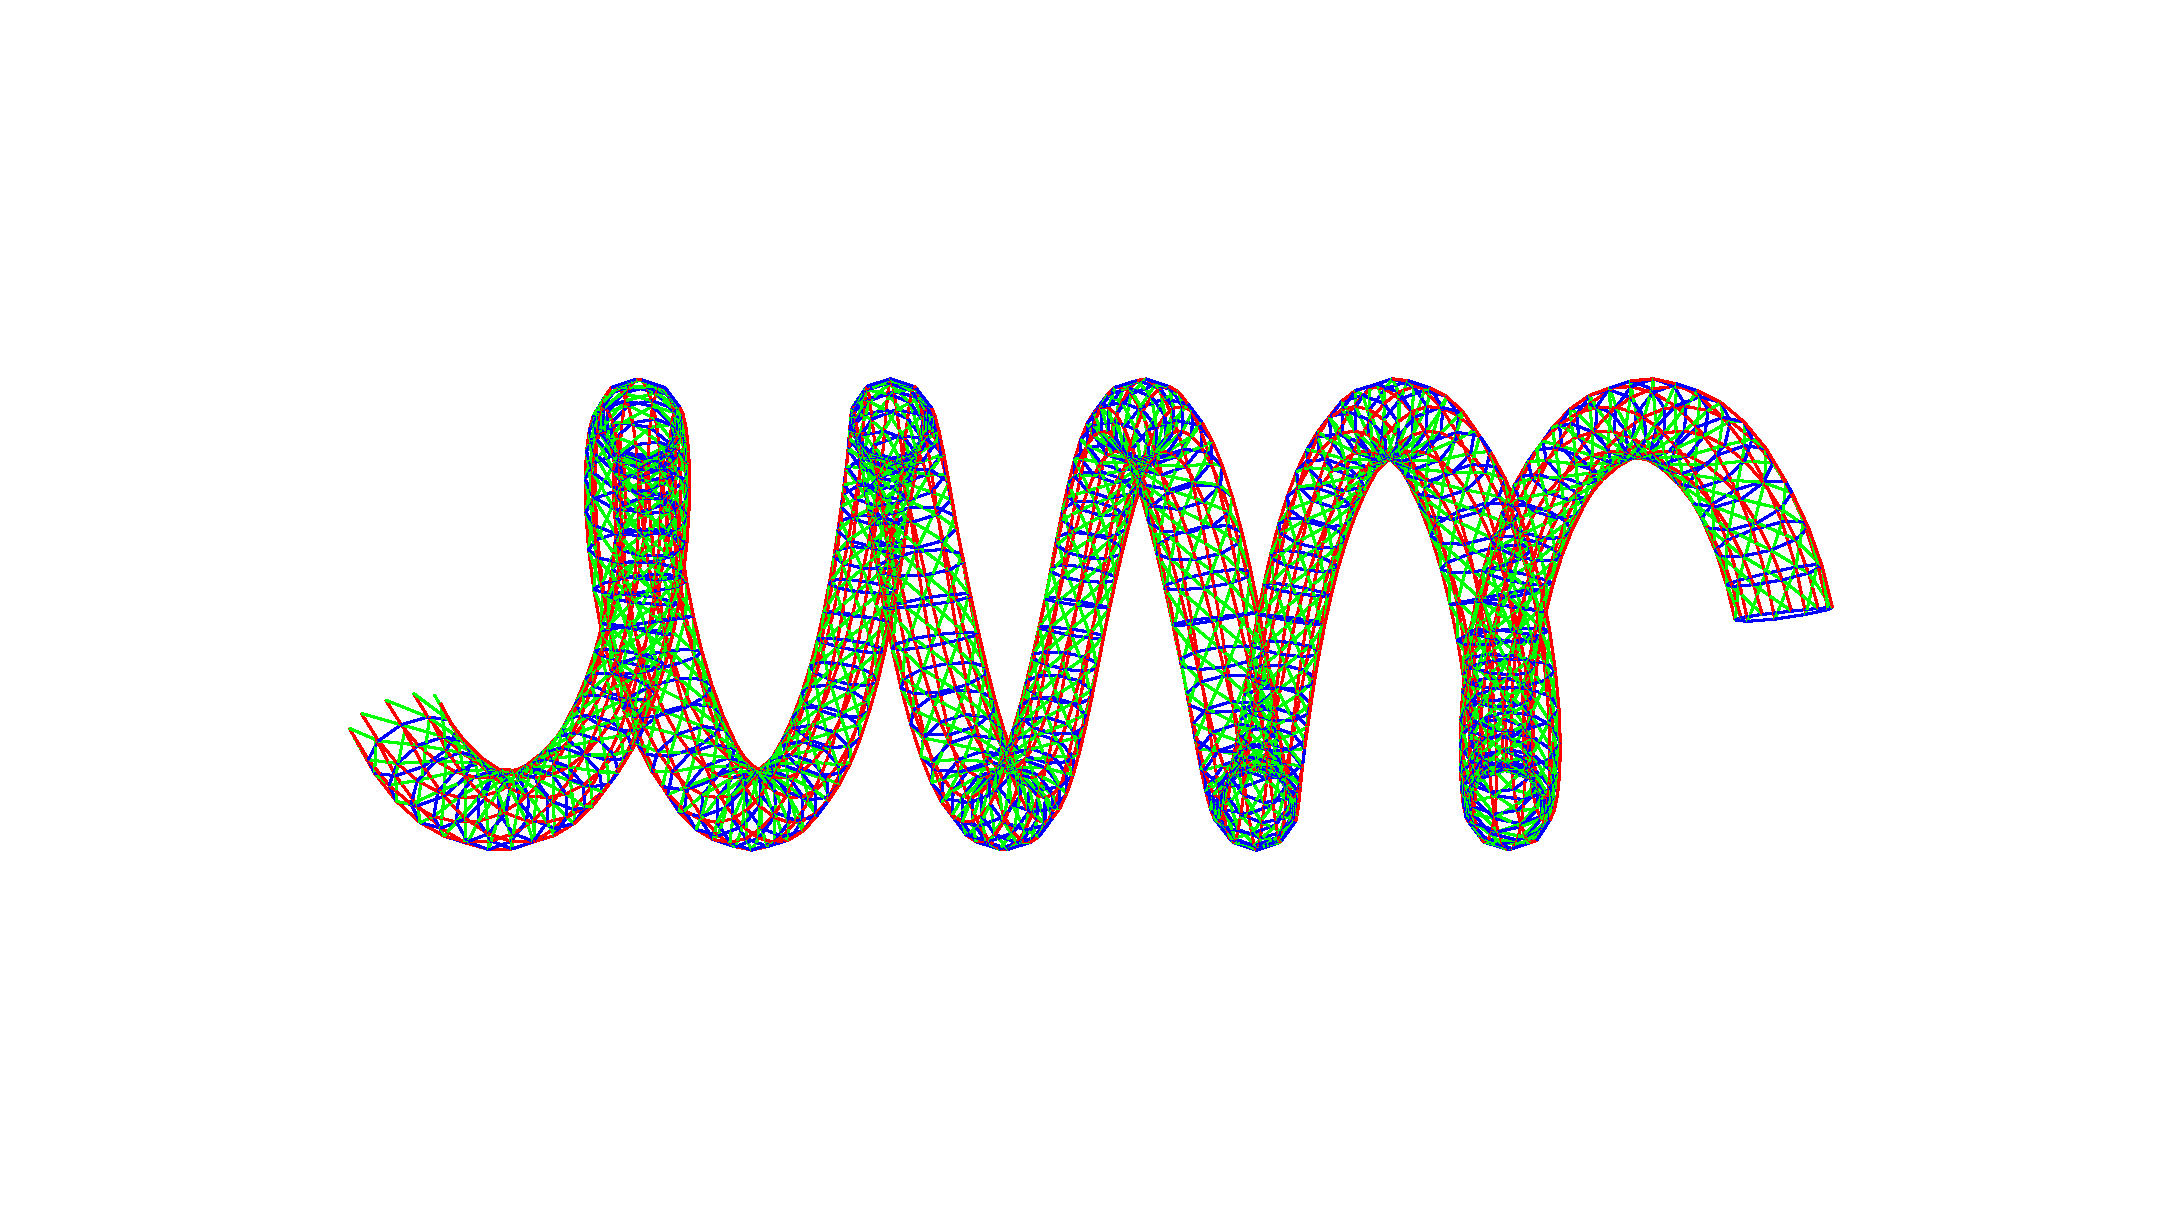
\includegraphics[width=5cm]{images/spiral-008}
   \end{latexonly}
   \begin{htmlonly}
     \htmladdimg{../images/spiral-007.png}
     \htmladdimg{../images/spiral-008.png}
   \end{htmlonly}  
   \caption{The spiral}
 \end{figure}


\subsection{Converting a Formex to a Finite Element model}
\label{subsec:femodel}

The \method{feModel()} method is important in exporting the geometry to finite element (FE) programs. A Formex often contains many points with (nearly) the same coordinates. In a finite element model, theses points have to be merged into a single nod, to express the continuity of the material. This is exactly what\method{feModel()} does. It returns a tuple of two numpy arrays (nodes,elems), where
\begin{itemize}
\item nodes is a float array with shape (?,3), containing the coordinates of the merged points (nodes),
\item elems is an integer array with shape (F.nelems(),F.nplex()), describing each element by a list of node numbers. The elements and their nodes are in the same order as in F.
\end{itemize}

\begin{verbatim}
>>> from simple import *
>>> F = Formex(pattern(Pattern['cube']))
>>> draw(F)
>>> nodes,elems = F.feModel()
>>> print 'Nodes',nodes
>>> print 'Elements',elems

Nodes
[[ 0.  0.  0.]
 [ 1.  0.  0.]
 [ 0.  1.  0.]
 [ 1.  1.  0.]
 [ 0.  0.  1.]
 [ 1.  0.  1.]
 [ 0.  1.  1.]
 [ 1.  1.  1.]]
Elements
[[0 1]
 [1 3]
 [3 2]
 [2 0]
 [0 4]
 [1 5]
 [3 7]
 [2 6]
 [4 5]
 [5 7]
 [7 6]
 [6 4]]
\end{verbatim}

The reverse operation of transforming a finite element model back into a Formex is quite simple: \code{Formex(nodes[elems])} will indeed be identical to the original F (within the tolerance used in merging of the nodes).

\begin{verbatim}
>>> G = Formex(nodes[elems])
>>> print allclose(F.f,G.f)
True
\end{verbatim}
The \code{allclose} funcion in the second line tests that all coordinates
in bopth arrays are the same, within a small tolerance.


%%%%%%%%%%%%%%%%%%%%%%%%%%%%%%%%%%%%%%%%%%%%%%%%%%%%%%%%%%%%%%%%%
\section{Assigning properties to geometry}
\label{sec:props}
\emph{As of version 0.7.1, the way to define properties for elements of the geometry has changed thoroughly. As a result, the proprty system has become much more flexibel and powerful, and can be used for Formex data structures as well as for TriSurfaces and Finite Element models.}

With properties we mean any data connected with some part of the geometry other than the coordinates of its points or the structure of points into elements.
Also, values that can be calculated purely from the coordinates of the points and the structure of the elements are usually not considerer properties.

Properties can e.g. define material characteristics, external loading and boundary conditions to be used in numerical simulations of the mechanics of a structure. The properties module includes some specific functions to facilitate assigning such properties. But the system is general enough to used it for any properties that you can think of.

Properties are collected in a \class{PropertyDB} object. Before you can store anything in this database, you need to create it. Usually, you will start with an empty database.
\begin{verbatim}
P = PropertyDB()
\end{verbatim}

\subsection{General properties}
\label{sec:general-properties}

Now you can start entering property records into the database. A property record is a lot like a Python dict object, and thus it can contain nearly anything. It is implemented however as a \class{CascadingDict} object, which means that the key values are strings and can also be used as attributes to address the value. Thus, if \Code{P} is a property record, then a field named \Code{key} can either be addressed as \Code{P['key']} or as \Code{P.key}. This implementation was choosen for the convenience of the user, but has no further advantages over a normal dict object. You should not use any of the methods of Python's dict class as key in a property record: it would override this method for the object.

The property record has four more reserved (forbidden) keys: \Code{kind}, \Code{tag}, \Code{set} and \code{nr}. The \Code{kind} and \Code{nr} should never be set nor changed by the user. \Code{kind} is used internally to distinguish among different kind of property records (see \ref{sec:node-properties}). It should only be used to extend the \class{PropertyDB} class with new kinds of properties, e.g. in subclasses. \Code{nr} will be set automatically to a unique record number. Some application modules use this number for identification and to create automatic names for property sets. 

The \Code{tag} and \Code{set} keys are optional fields and can be set by the user. They should however only be used for the purposes explained hereafter, because they have a special meaning for the database methods and application modules. The \Code{set} can be used to specify a list of integer numbers identifying a collection of elements of the geometry for which the current property is valid. Absence of the \Code{set} means that the property is assigned to all elements. The \Code{tag} field can be used to attach an identification string to the property record. THis string can be as complex as the user wants and its interpretation is completely left to the user. The \class{ProeprtyDB} class just provides an easy way to select the records by their \Code{tag} name or by a set of tag names.  
So let's create a property record in our database. The \Code{Prop()} method does just that. It also returns the property record, so you can directly use it further in your code.
\begin{verbatim}
>>> Stick = P.Prop(colour='green',name='Stick',weight=25, \
        comment='This could be anything: a gum, a frog, a usb-stick,...'})
>>> print Stick

  color = green
  comment = This could be anything: a gum, a frog, a usb-stick,...
  nr = 0
  name = Stick
  weight = 25
\end{verbatim}
Notice the auto-generated \Code{nr} field. Here's another example, with a tag:
\begin{verbatim}
>>> author = P.Prop(tag='author',name='Alfred E Neuman',\
        address=CascadingDict({'street':'Krijgslaan', 'city':'Gent','country':'Belgium'}))
>>> print author

  nr = 1
  tag = author
  name = Alfred E Neuman
  address = 
    city = Gent
    street = Krijgslaan
    country = Belgium
\end{verbatim}
This example shows that record values can be complex structured objects.
Notice how the \class{CascadingDict} object is by default printed in a very readible layout, offsetting each lower level dictionary two more postions to the right. 

The \class{CascadingDict} has yet another fine characteristic: if an attribute is not found in the toplevel, all values that are instances of \class{CascadingDict} or \class{Dict} (but not the normal Python dict) will be searched for the attribute. If needed, this searching is even repeated in the values of the next levels, and further on, thus cascading though all levels of \class{CascadingDict} structures until the attribute can eventually be found. The cascading does not proceed through values in a \class{Dict}.

If you set an attribute of a \class{CascadingDict}, it is always set in the toplevel. If you want to change lower level attributes, you need to use the full path to it.
\begin{verbatim}
>>> print author.street
  Krijgslaan
>>> author.street = 'Voskenslaan'
>>> print author.street
  Voskenslaan
>>> print author.address.street
  Krijgslaan
>>> author.address.street = 'Wiemersdreef'
>>> print author.address.street
  Wiemersdreef
>>> author = P.Prop(tag='author',alias='John Doe',\
        address={'city': 'London', 'street': 'Downing Street 10', 'country': 'United Kingdom'})
>>> print author

  nr = 2
  tag = author
  alias = John Doe
  address = {'city': 'London', 'street': 'Downing Street 10', 'country': 'United Kingdom'} 
\end{verbatim}

In the examples above, we have given a name to the created property records, so that we could address them in the subsequent print and field assigment statements. In most cases however, it will be impractical and unnecessary to give your records a name. They all are recorded in the \class{PropertyDB} database, and will exist as long as the database variable lives. There should be away though to request selected data from that database. The \method{getProp()} method returns a list of records satisfying some conditions. The examples below show how it can be used.

\begin{verbatim}
>>> for p in P.getProp(rec=[0,2]):
        print p.name
Stick
John Doe
>>>  for p in P.getProp(tag=['author']):
        print p.name
None
John Doe
>>>  for p in P.getProp(attr=['name']):
        print p.nr
0
2
>>>  for p in P.getProp(tag=['author'],attr=['name']):
        print p.name
John Doe
\end{verbatim}
The first call selects records by number: either a single record number or a list of numbers can be specified. The second method selects records based on the value of their tag field. Again a single tag value or a list of values can be specified. Only those records having a 'tag' filed matching any of the values in the list will be returned. The third selection method is based on the existence of some attribute names in the record. Here, always a list of attribute names is required. Records are returned that posess all the attributes in the list, independent from the value of those attributes. If needed, the user can add a further filtering based on the attribute values. Finally, as is shown in the last example, all methods of record selection can be combined. Each extra condition will narrow the selection further down.


\subsection{Specialized property records}
\label{sec:special-properties}

The property system presented above allows for recording any kind of values. In many situations however we will want to work with a specialised and limited set of attributes. The main developers of \pyf e.g. often use the program to create geometrical models of structures of which they want to analyse the mechanical behavior. These numerical simulations (FEA, CFD) require specific data that support the introduction of specialised property records. Currently there are two such property record types: node properties (see \ref{sec:node-properties}), which are attributed to a single point in space, and element properties (\ref{sec:elem-properties}), which are attributed to a structured collection of points.

Special purpose properties are distincted by their \Code{kind} field. General property records have {\Code{kind=''}, node properties haven {\Code{kind='n'} and 
 {\Code{kind='e'} is set for element properties. Users can create their own specialised property records by using other value for the \Code{kind} parameter.


\subsection{Node properties}
\label{sec:node-properties}

Node properties are created with the \method{nodeProp} method, rather than the general \method{Prop}. The \Code{kind} field does not need to be set: it will be done automatically. When selecting records using the \method{getProp} method, add a \Code{kind='n'} argument to select only node properties.

Node properties will recognize some special field names and check the values for consistency. Application plugins such as the Abaqus input file generator depend on these property structure, so the user should not mess with them. Currently, the following attributes are in use:
\begin{description}
 \item [cload] A concentrated load at the node. This is a list of 6 items: three force components in axis directions and three force moments around the axes: \Code{[F_0, F_1, F_2, M_0, M_1, M_2]}. 
 \item [bound] A boundary condition for the nodal displacement components. This can be defined in 2 ways:
     \begin{itemize}
     \item as a list of 6 items \Code{[ u_0, u_1, u_2, r_0, r_1, r_2 ]}. These items have 2 possible values:
         \begin{description}
         \item [0] The degree of freedom is not restrained.
         \item [1] The degree of freedom is restrained.
         \end{description}
     \item as a string. This string is a standard boundary type. Abaqus will recognize the following strings:
         \begin{itemize}
         \item PINNED 
         \item ENCASTRE
         \item XSYMM
         \item YSYMM
         \item ZSYMM
         \item XASYMM
         \item YASYMM 
         \item ZASYMM
         \end{itemize} 
     \end{itemize}
 \item [displacement] Prescribed displacements. This is a list of tuples (i,v), where i is a DOF number (1..6) and v is the prescribed value for that DOF. 
 \item [coords] The coordinate system which is used for the definition of cload, bound and displ fields. It should be a \class{CoordSys} object.
\end{description}

Some simple examples:
\begin{verbatim}
    P.nodeProp(cload=[5,0,-75,0,0,0])
    P.nodeProp(set=[2,3],bound='pinned')
    P.nodeProp(5,displ=[(1,0.7)])
\end{verbatim}
The first line sets a concentrated load all the nodes, the second line sets a boundary condition 'pinned' on nodes 2 and 3. The third line sets a prescribed displacement on node 5 with value 0.7 along the first direction.
The first positional argument indeed corresponds to the 'set' attribute.

Often the properties are computed and stored in variables rather than entered directly.
\begin{verbatim}
    P1 = [ 1.0,1.0,1.0, 0.0,0.0,0.0 ]
    P2 = [ 0.0 ] * 3 + [ 1.0 ] * 3 
    B1 = [ 1 ] + [ 0 ] * 5
    CYL = CoordSystem('cylindrical',[0,0,0,0,0,1])
    P.nodeProp(bound=B1,csys=CYL)
\end{verbatim}
The first two lines define two concentrated loads: \code{P1} consists of three point loads in each of the coordinate directions; P2 contains three force moments around the axes.
The third line specifies a boundary condition where the first DOF (usually displacement in $x$-direction) is constrained, while the remaining 5 DOF's are free.
The next line defines a local coordinate system, in this case a cylindrical coordinate system with axis pointing from point \code{[0.,0.,0.]} to point \code{[0.,0.,1.]}. The last line 

To facilitate property selection, a tag can be added.
\begin{verbatim}
    nset1 = P.nodeProp(tag='loadcase 1',set=[2,3,4],cload=P1).nr
    P.nodeProp(tag='loadcase 2',set=Nset(nset1),cload=P2)
\end{verbatim}
The last two lines show how you can avoid duplication of sets in mulitple records. The same set of nodes should receive different concentrated load values for different load cases. The load case is stored in a tag, but duplicating the set definition could become wasteful if the sets are large. Instead of specifying the node numbers of the set directly, we can pass a string setting a set name.
Of course, the application will need to know how to interprete the set names.
Therefore the property module provides a unified way to attach a unique set name to each set defined in a property record. The name of a node property record set can be obtained with the function \Code{Nset(nr)}, where nr is the record number. In the example above, that value is first recorded in \Code{nset1} and then used in the last line to guarantee the use of the same set as in the property above.


\subsection{Element properties}
\label{sec:elem-properties}


The \method{elemProp} method creates element properties, which will have their \code{kind} attribute set to 'e'. When selecting records using the \method{getProp} method, add the \Code{kind='e'} argument to get element properties.

Like node properties, element property records have a number of specialize fields. Currently, the following ones are recognized by the Abaqus input file generatr.
\begin{description}
 \item [eltype] This is the single most import element property. It sets the element type that will be used during the analysis. Notice that a Formex object also may have an \code{eltype} attribute; that one however is only used to describe the type of the geometric elements involved. The element type discussed here however may also define some other characteristics of the element, like the number and type of degrees of freedom to be used in the analysis or the integration rules to be used. What element types are available is dependent on the analysis package to be used. Currently, \pyf does not do any checks on the element type, so the simulation program's own element designation may be used.
 \item[section] The section properties of the element. This should be an \class{ElemSection} instance, grouping material properties (like Young's modulus) and geometrical properties (like plate thickness or beam section).
 \item[dload] A distributed load acting on the element. The value is an \class{ElemLoad} instance. Currently, this can include a label specifying the type of distributed loading, a value for the loading, and an optional amplitude curve for specifying the variation of a time dependent loading.  
\end{description}


\emph{The rest of this section is obsolete}

An elemsection can hold the following sub-properties:
\begin{description}
\item [section] The section properties of the element. This can be a dictionary or a string. The required data in this dict depends on the sectiontype. 
\item [material] The element material properties. This can be a dictionary which holds these properties or a string which can be used to search a material database. 
\item [sectiontype] The sectiontype of the element. 
\item [orientation]  A list [First direction cosine, second direction cosine, third direction cosine] of the first beam section axis. This allows to change the orientation of the cross-section.
\end{description}

An element load can hold the following sub-properties:
\begin{description}
\item [magnitude] The magnitude of the distibuted load.
\item [loadlabel] The distributed load type label.
\end{description}

The overview of the current property database structure is:
\begin{itemize}
\item[-] Prop
    \begin{itemize}
    \item[-] set
    \item[-] tag
    \end{itemize}
\item[-] nodeProp
    \begin{itemize}
    \item[-] cload
    \item[-] bound
    \item[-] displ
    \item[-] csys
    \end{itemize}
\item[-] elemProp 
    \begin{itemize}
    \item[-] eltype
    \item[-] section
        \begin{itemize}
        \item[-] section
        \item[-] material
        \item[-] sectiontype
        \item[-] orientation
        \end{itemize}
    \item[-] load
        \begin{itemize}
        \item[-] label
        \item[-] value
        \end{itemize}
    \end{itemize}
\end{itemize}

\begin{verbatim}
>>> vert = ElemSection('IPEA100', 'steel')
>>> hor = ElemSection({'name':'IPEM800','A':951247,'I':CascadingDict(
{'Ix':1542,'Iy':6251,'Ixy':352})}, {'name':'S400','E':210,'fy':400})
>>> q = ElemLoad(magnitude=2.5, loadlabel='PZ')
>>> top = ElemProperty(1,hor,[q],'B22')
>>> column = ElemProperty(2,vert, elemtype='B22')
>>> diagonal = ElemProperty(4,hor,elemtype='B22')

>>> print 'elemproperties'
>>> for key, item in elemproperties.iteritems():
>>>     print key, item    

elemproperties
1
  elemtype = B22
  elemload = [CascadingDict({'magnitude': 2.5, 'loadlabel': 'PZ'})]
  elemsection =
    section =
      A = 951247
      I =
        Iy = 6251
        Ix = 1542
        Ixy = 352
      name = IPEM800
    material =
      fy = 400
      E = 210
      name = S400
    orientation = None
    sectiontype = general
2
  elemtype = B22
  elemload = None
  elemsection =
    section =
      torsional_rigidity = 1542
      name = IPEA100
      moment_inertia_22 = 1140000
      cross_section = 878
      moment_inertia_11 = 1412000
      moment_inertia_12 = 1254
    material =
      shear_modulus = 25
      young_modulus = 210
      name = steel
    orientation = None
    sectiontype = general
4
  elemtype = B22
  elemload = None
  elemsection =
    section =
      A = 951247
      I =
        Iy = 6251
        Ix = 1542
        Ixy = 352
      name = IPEM800
    material =
      fy = 400
      E = 210
      name = S400
    orientation = None
    sectiontype = general
\end{verbatim}


%
\section{Exporting to finite element programs}


%
%%% Local Variables: 
%%% mode: latex
%%% TeX-master: "pyformex"
%%% End: 
